\chapter{LANDASAN TEORI}

Bab ini menjelaskan landasan teori yang menjadi dasar ilmiah dalam penelitian.
Landasan teori tidak menjelaskan implementasi penelitian yang dilakukan oleh
penulis, melainkan menjelaskan konsep, teori, metode, dan penelitian terdahulu
yang relevan dengan topik penelitian.

Struktur Bab ini biasanya terdiri dari:
\begin{itemize}
\item Konsep dasar yang berkaitan dengan topik penelitian
\item Teori atau metode yang digunakan dalam penelitian
\item Penelitian terdahulu (State of The Art)
\item Analisis research gap
\end{itemize}

Semua gambar, tabel, maupun persamaan yang ditampilkan pada bab ini harus
dijelaskan dalam teks dan dirujuk menggunakan perintah \texttt{\textbackslash ref}.
Tidak diperbolehkan menampilkan gambar atau tabel tanpa penjelasan dalam teks.

%%%%%%%%%%%%%%%%%%%%%%%%%%%%%%%%%%%%%
\section{(Contoh Section) Konsep Dasar Web Application}
%%%%%%%%%%%%%%%%%%%%%%%%%%%%%%%%%%%%%

Bagian ini menjelaskan konsep dasar yang berkaitan dengan sistem atau teknologi
yang digunakan dalam penelitian. Penjelasan harus didukung dengan referensi
ilmiah dari jurnal, buku, atau prosiding konferensi.

Sebagai contoh, web application merupakan sistem perangkat lunak yang berjalan
pada web server dan dapat diakses melalui browser menggunakan protokol HTTP.
Arsitektur web application umumnya terdiri dari tiga komponen utama yaitu
client, server, dan database \parencite{llama2024}.

%%%%%%%%%%%%%%%%%%%%%%%%%%%%%%%%%%%%%
\section{(Contoh Section) Algoritma Enhancement}
%%%%%%%%%%%%%%%%%%%%%%%%%%%%%%%%%%%%%

Bagian ini menjelaskan teori mengenai algoritma enhancement yang menjadi dasar
dari penelitian. Penjelasan harus bersifat konseptual dan teoritis.

Sebagai contoh, algoritma enhancement digunakan untuk meningkatkan kualitas
data atau performa sistem melalui proses optimasi tertentu.

\subsection{(Contoh subsection) Jenis Algoritma Enhancement}

Ini contoh numbering / itemize:

\begin{itemize}
\item Image Enhancement Algorithm
\item Feature Enhancement Algorithm
\item Performance Optimization Algorithm
\end{itemize}

\subsubsection{(Contoh Section) Struktur Section, Subsection, dan Subsubsection}

Dalam penulisan dokumen ilmiah menggunakan \LaTeX, struktur pembahasan dapat
diatur secara sistematis menggunakan perintah \texttt{section},
\texttt{subsection}, dan \texttt{subsubsection}. Struktur ini berfungsi untuk
mengorganisasi pembahasan dari topik yang bersifat umum hingga lebih spesifik
secara hierarkis.

Secara umum, hierarki struktur penulisan dapat digambarkan sebagai berikut:

\begin{itemize}
\item \textbf{Section}
\item \quad -- \textbf{Subsection}
\item \quad \quad -- \textbf{Subsubsection}
\end{itemize}

Dengan struktur tersebut, penulis dapat membagi pembahasan secara sistematis
tanpa perlu membuat penomoran manual seperti yang biasa dilakukan pada
perangkat pengolah kata (misalnya Microsoft Word). Sistem penomoran akan
dihasilkan secara otomatis oleh \LaTeX.

\subsubsection{(Contoh Section) Penjelasan Section, Subsection, dan Subsubsection}

Berikut penjelasan mengenai fungsi masing-masing struktur dalam penulisan
dokumen ilmiah:

\begin{itemize}
\item \textbf{Section (\texttt{\textbackslash section})}

Digunakan untuk membagi pembahasan utama dalam suatu bab. Section biasanya
mewakili topik besar yang akan dijelaskan dalam bab tersebut.

\item \textbf{Subsection (\texttt{\textbackslash subsection})}

Digunakan untuk membagi pembahasan pada section menjadi bagian yang lebih
spesifik. Subsection biasanya menjelaskan komponen atau aspek tertentu dari
topik utama yang dibahas pada section.

\item \textbf{Subsubsection (\texttt{\textbackslash subsubsection})}

Digunakan untuk memberikan penjelasan yang lebih rinci dari subsection.
Struktur ini umumnya digunakan untuk menjelaskan detail teknis, tahapan,
atau komponen yang lebih spesifik dari suatu konsep.
\end{itemize}

Penggunaan struktur ini membantu menjaga konsistensi penulisan serta
mempermudah pembaca dalam memahami alur pembahasan penelitian.

\subsection{Tahapan Algoritma Enhancement}

Tahapan umum dalam algoritma enhancement dapat digambarkan seperti pada
Gambar \ref{fig:enhancement-flow}.

\begin{figure}[H]
\centering
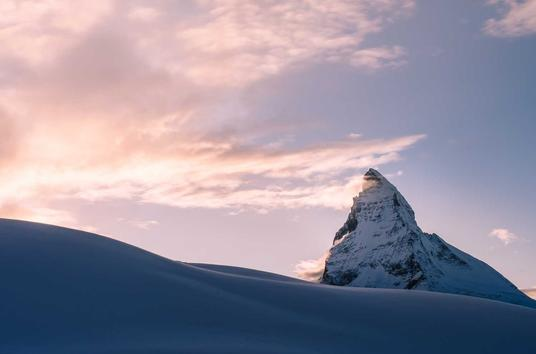
\includegraphics[width=0.7\textwidth]{images/lorem-picsum.jpg}
\caption{Alur umum proses enhancement}
\label{fig:enhancement-flow}
\end{figure}

Berdasarkan Gambar \ref{fig:enhancement-flow}, proses enhancement umumnya
dimulai dari proses preprocessing data, dilanjutkan dengan proses optimasi,
dan diakhiri dengan evaluasi performa sistem.

%%%%%%%%%%%%%%%%%%%%%%%%%%%%%%%%%%%%%
\section{State of the Art Penelitian Terdahulu}
%%%%%%%%%%%%%%%%%%%%%%%%%%%%%%%%%%%%%

Bagian ini menjelaskan penelitian-penelitian sebelumnya yang relevan dengan
topik penelitian. Tujuan dari bagian ini adalah untuk menunjukkan perkembangan
penelitian pada bidang yang sama serta menemukan kesenjangan penelitian
(research gap).

Penelitian terdahulu biasanya dirangkum dalam bentuk tabel agar memudahkan
analisis perbandingan antar penelitian.

Contoh tabel State of the Art dapat dilihat pada Tabel \ref{tab:sota}.

\begin{table}[H]
\centering
\begin{tabular}{p{3cm} p{3cm} p{3cm} p{4cm}}
\toprule
Author & Kekurangan & Kelebihan & Gap Penelitian \\
\midrule

\cite{rag2023} &
Model memiliki akurasi rendah pada dataset besar &
Metode yang digunakan cukup sederhana dan mudah diimplementasikan &
Belum dilakukan optimasi menggunakan algoritma enhancement

\\

\cite{author2021} &
Dataset yang digunakan terbatas &
Menggunakan metode deep learning modern &
Belum dilakukan integrasi dengan sistem web application

\\

\cite{author2022} &
Kompleksitas komputasi tinggi &
Akurasi sistem meningkat secara signifikan &
Belum ada evaluasi performa pada sistem real-time

\\

\bottomrule
\end{tabular}

\caption{Perbandingan penelitian terdahulu (State of the Art)}
\label{tab:sota}
\end{table}

Berdasarkan Tabel \ref{tab:sota}, dapat dilihat bahwa penelitian sebelumnya
memiliki beberapa keterbatasan seperti keterbatasan dataset, kompleksitas
komputasi, serta belum adanya integrasi dengan sistem web application.

%%%%%%%%%%%%%%%%%%%%%%%%%%%%%%%%%%%%%
\section{Contoh: Analisis Research Gap}
%%%%%%%%%%%%%%%%%%%%%%%%%%%%%%%%%%%%%

Berdasarkan analisis penelitian terdahulu pada Tabel \ref{tab:sota}, dapat
diidentifikasi beberapa research gap yang menjadi dasar dilakukannya penelitian
ini, antara lain:

\begin{enumerate}
\item Belum adanya penelitian yang mengintegrasikan algoritma enhancement
dengan sistem web application secara optimal.
\item Belum adanya evaluasi performa sistem pada skenario penggunaan nyata.
\item Masih terbatasnya penelitian yang memanfaatkan dataset dengan skala besar.
\end{enumerate}

Research gap tersebut menjadi dasar bagi penelitian ini untuk mengembangkan
metode yang mampu meningkatkan performa sistem web application melalui
pendekatan algoritma enhancement yang lebih efektif.

%%%%%%%%%%%%%%%%%%%%%%%%%%%%%%%%%%%%%
\section{Contoh: Kerangka Konseptual Penelitian}
%%%%%%%%%%%%%%%%%%%%%%%%%%%%%%%%%%%%%

Kerangka konseptual penelitian menggambarkan hubungan antara teori,
metode, dan permasalahan penelitian.

Ilustrasi kerangka konseptual dapat dilihat pada Gambar \ref{fig:framework}.

\begin{figure}[H]
\centering
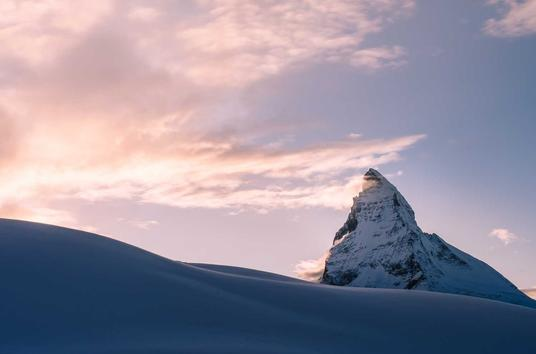
\includegraphics[width=0.8\textwidth]{images/lorem-picsum.jpg}
\caption{Kerangka konseptual penelitian}
\label{fig:framework}
\end{figure}

Gambar \ref{fig:framework} menunjukkan hubungan antara teori web application,
algoritma enhancement, serta metode evaluasi yang digunakan dalam penelitian.